% ****************************************************************************************************
\chapter{Konzept und Implementierung} \label{ch:concept}
Aufbauend auf \autoref{ch:background} und \autoref{ch:sota} wird nun ein Konzept zum Erkennen von landwirtschaftlichen Maschinen vorgestellt.
% Dazu wird zunächst der für das Konzept erwartete Aufbau am Windrad und des Prototypen beschrieben  \textit{(Business Understanding)}.
In \autoref{ch5:arch} wird eine Architektur zur Lösung des Problems eingeführt.
Die anschließenden Abschnitte beschreiben die einzelnen Bausteine der Architektur.
\autoref{ch5:alarm} gibt erste Ideen für das Alarmsystem, welche bei der Entwicklung beachtet werden können.


% ****************************************************************************************************
\section{Architektur}
\label{ch5:arch}

In \autoref{ch5:components} werden die einzelnen Komponenten für das System dargestellt.
Wie deren konzeptionelle Zusammenarbeit aussieht, ist in \autoref{ch5:concept} erläutert.
Abschließend werden in \autoref{ch5:tech} die jeweiligen Frameworks für die benötigten Arbeitsschritte vorgestellt.


% ****************************************************************************************************
\subsection{Komponenten} \label{ch5:components}
In \autoref{ch5:fig:components} sind die relevanten Komponenten zu sehen.
Dabei erhält das System von einer Kamera Bildsequenzen, aus welchen mittels Background Subtraction die Bildbereiche extrahiert werden können, in denen Bewegungen festgestellt wurden.

Für diese Bereiche entscheidet ein Klassifizierer über die jeweilige Klasse.
In diesem Anwendungsfall sind das die Klassen \SC{Traktor} und \SC{Andere}.

Die Alarmlogik erhält daraufhin die Vorhersagen und entscheidet, ob ein Alarm gegeben werden soll oder nicht.

\begin{figure}[ht]
    \begin{small}
        \begin{center}
            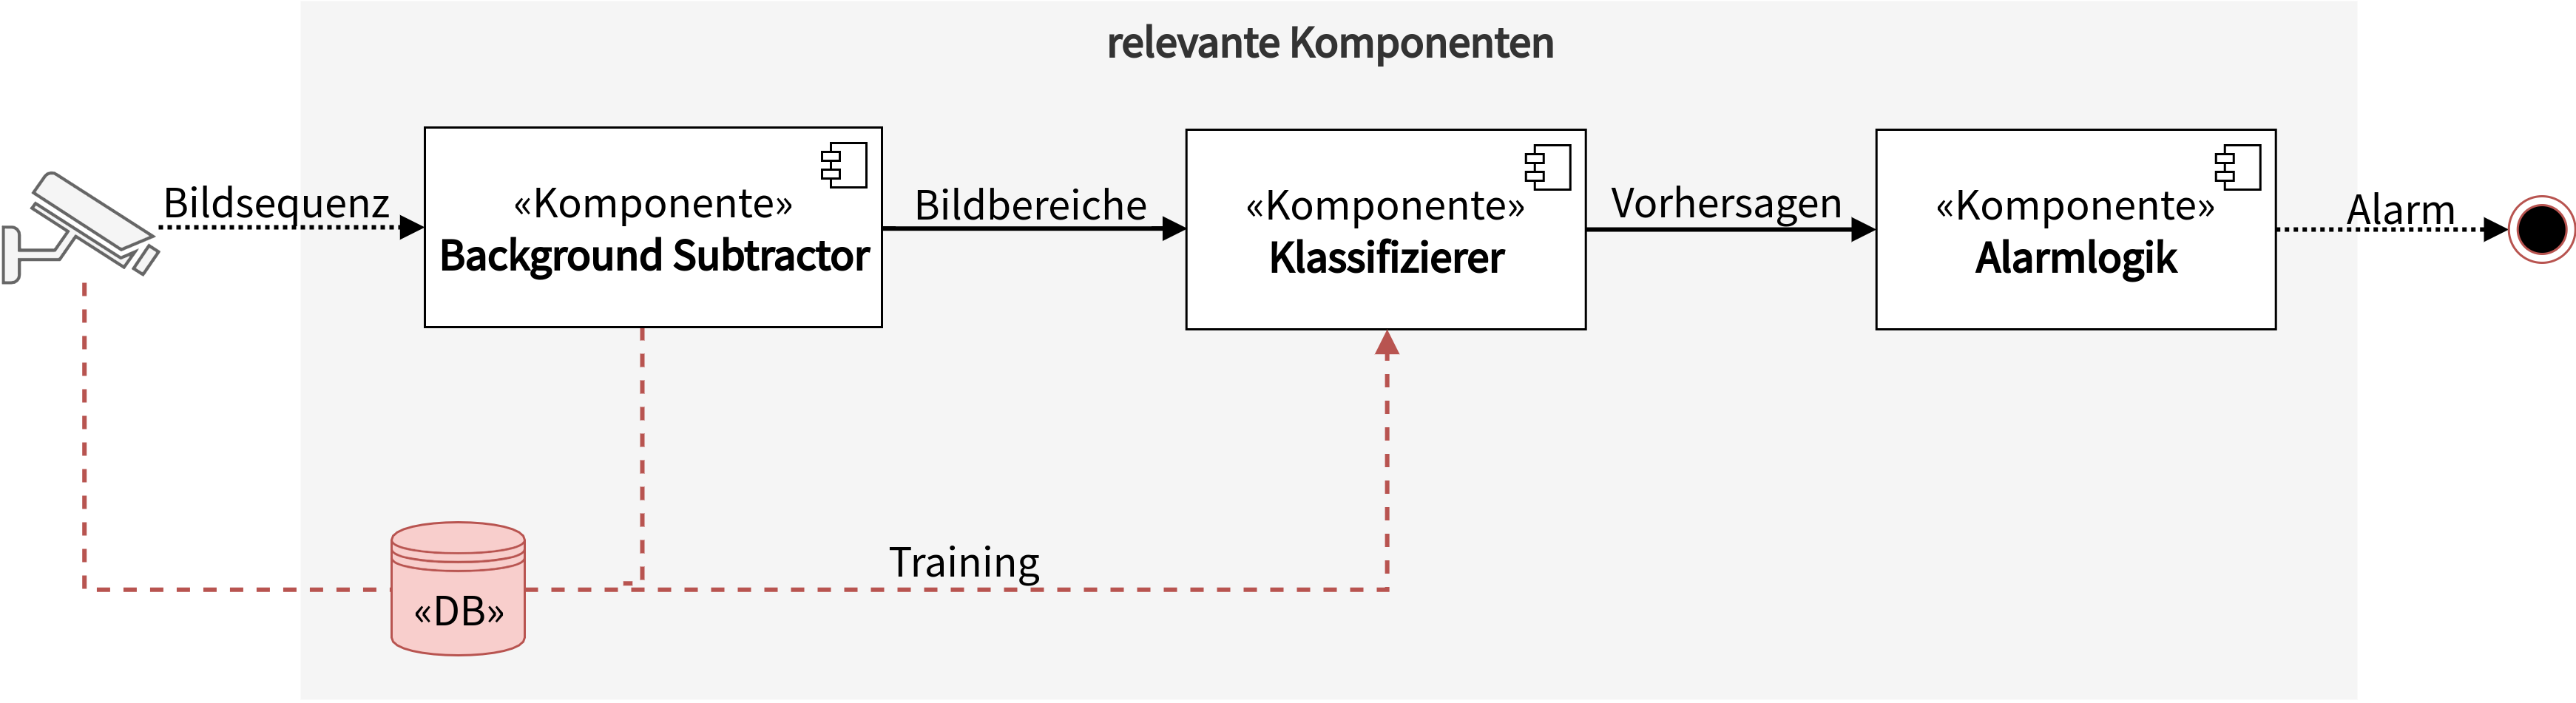
\includegraphics[width=0.95\textwidth]{figures/architecture/components.png}
        \end{center}
        \caption{Komponentensicht}
        \label{ch5:fig:components}
    \end{small}
\end{figure}

Beim Klassifizierer handelt es sich um ein \ac{CNN}.
Daher müssen zuvor Trainingsdaten gesammelt werden, welche in einer Datenbank abgelegt werden.

\subsection{Konzeptionelle Verarbeitung} \label{ch5:concept}
Um ein besseres Verständnis für die Interaktion der einzelnen Komponenten zu erhalten, sind deren Ergebnisse in \autoref{ch5:fig:dataflow} visualisiert.

Verarbeitet das System drei Bildsequenzen (1), wird für jede Sequenz ein Background Modell erstellt und eine Background Subtraction ausgeführt.
Auf der draus entstehenden Vordergrundmaske kann dann eine Blobanalyse durchgeführt werden (2).
Dabei wird geprüft, ob die gefundenen \acp{ROI} eine gewisse Größe aufweisen.

Resultat der bisherigen Schritte sind die Vordergrundobjekte (3).
Ist noch kein \ac{CNN} trainiert, müssen die Vordergrundobjekte vorerst gelabelt und in einer Datenbank dementsprechend hinterlegt werden (4).
Anschließend kann das \ac{CNN} auf den Daten trainiert werden (5).

In der Inferenzphase wird das trainierte \ac{CNN} eingesetzt, um ungesehene Daten zu klassifizieren (6).
Es handelt sich hierbei also um neue Vordergrundobjekte.
Je nach Ausgabe des \ac{CNN}s reagiert die Alarmlogik (7).

\begin{figure}[ht]
    \begin{small}
        \begin{center}
            \includegraphics[width=0.95\textwidth]{figures/architecture/concept.png}
        \end{center}
        \caption{Konzept - von der Eingabe zum Traktor}
        \label{ch5:fig:dataflow}
    \end{small}
\end{figure}

\bigskip
Mit diesem Konzept werden nur sich bewegende Objekte erkannt und klassifiziert.
Das ist allerdings keine Einschränkung für den Anwendungsfall, da Traktoren nicht plötzlich mitten auf dem Acker stehen und sich nicht mehr bewegen.
% Und wenn doch, würden durch seine reine Anwesenheit keine Kleintiere - solange nicht bereits dazu konditioniert - aufgescheucht, welche die Vögel anlocken würden. \\

Ebenso ist das Erstellen der Trainingsdaten auf diese Weise relativ schnell, da nicht für jedes Bild händisch Bounding Boxes mit entsprechender Klasse erstellt werden müssen.

% ****************************************************************************************************
\subsection{Datenfluss \& verwendete Technologien} \label{ch5:tech}
In \autoref{ch5:fig:technologies} ist der Datenfluss und die jeweils verwendete Technologie der Aufgabe zu sehen.
Unterteilt ist der Datenfluss in Inferenz und Training.
In beiden Fällen werden die Eingangsbilder mittels \SC{OpenCV} vorverarbeitet (engl. \IT{preprocessed}). Das Bild wird gelesen, eine Background Subtraction wird ausgeführt und die gefundenen \acp{ROI} werden auf Größe analysiert.

\bigskip
Der nächste Schritt für das Training beinhaltet einen (menschlichen) Akteur, der die gefunden \acp{ROI} klassifiziert (engl. label).
Die Daten werden dann in unterschiedliche Datensätze geteilt (mehr dazu in \autoref{ch5:data}).

Auf diesen Daten wird daraufhin ein \ac{CNN} trainiert, das lernt die Bilder zu klassifizieren.
Implementiert wird mittels \SC{TensorFlow}, welches die darauf aufbauende API \SC{Keras} mit ausliefert.
Es wird die GPU Variante zu verwendet, welche dank \SC{CUDA} das Trainieren auf der Grafikkarte stark beschleunigt.
Zur Evaluation des Modells wird \SC{TensorBoard} verwendet, welches die Ergebnisse visualisiert.

\bigskip
Bevor das \ac{CNN} letztendlich genutzt wird, wird es mit \SC{TensorRT} optimiert.
Dabei wird es auf die Grafikkarte zugeschneidert; Layer, die keine Auswirkung auf das Ergebnis haben, werden entfernt und die Gewichte werden quantisiert, also weniger Bits für die Floating Point Nachkommastellen verwendet.

In der Inferenzphase werden die Bildbereiche vom optimiertem \ac{CNN} klassifiziert.
Wichtig ist hierbei, dass die Bilder den identischen Vorverarbeitungsschritten unterlaufen.
Eine Stolperfalle bildet das Laden der Bilder, da \SC{OpenCV} standardmäßig Bilder im BGR-Format und \SC{TensorFlow} im RGB-Format verarbeitet.

\begin{figure}[ht]
    \begin{small}
        \begin{center}
            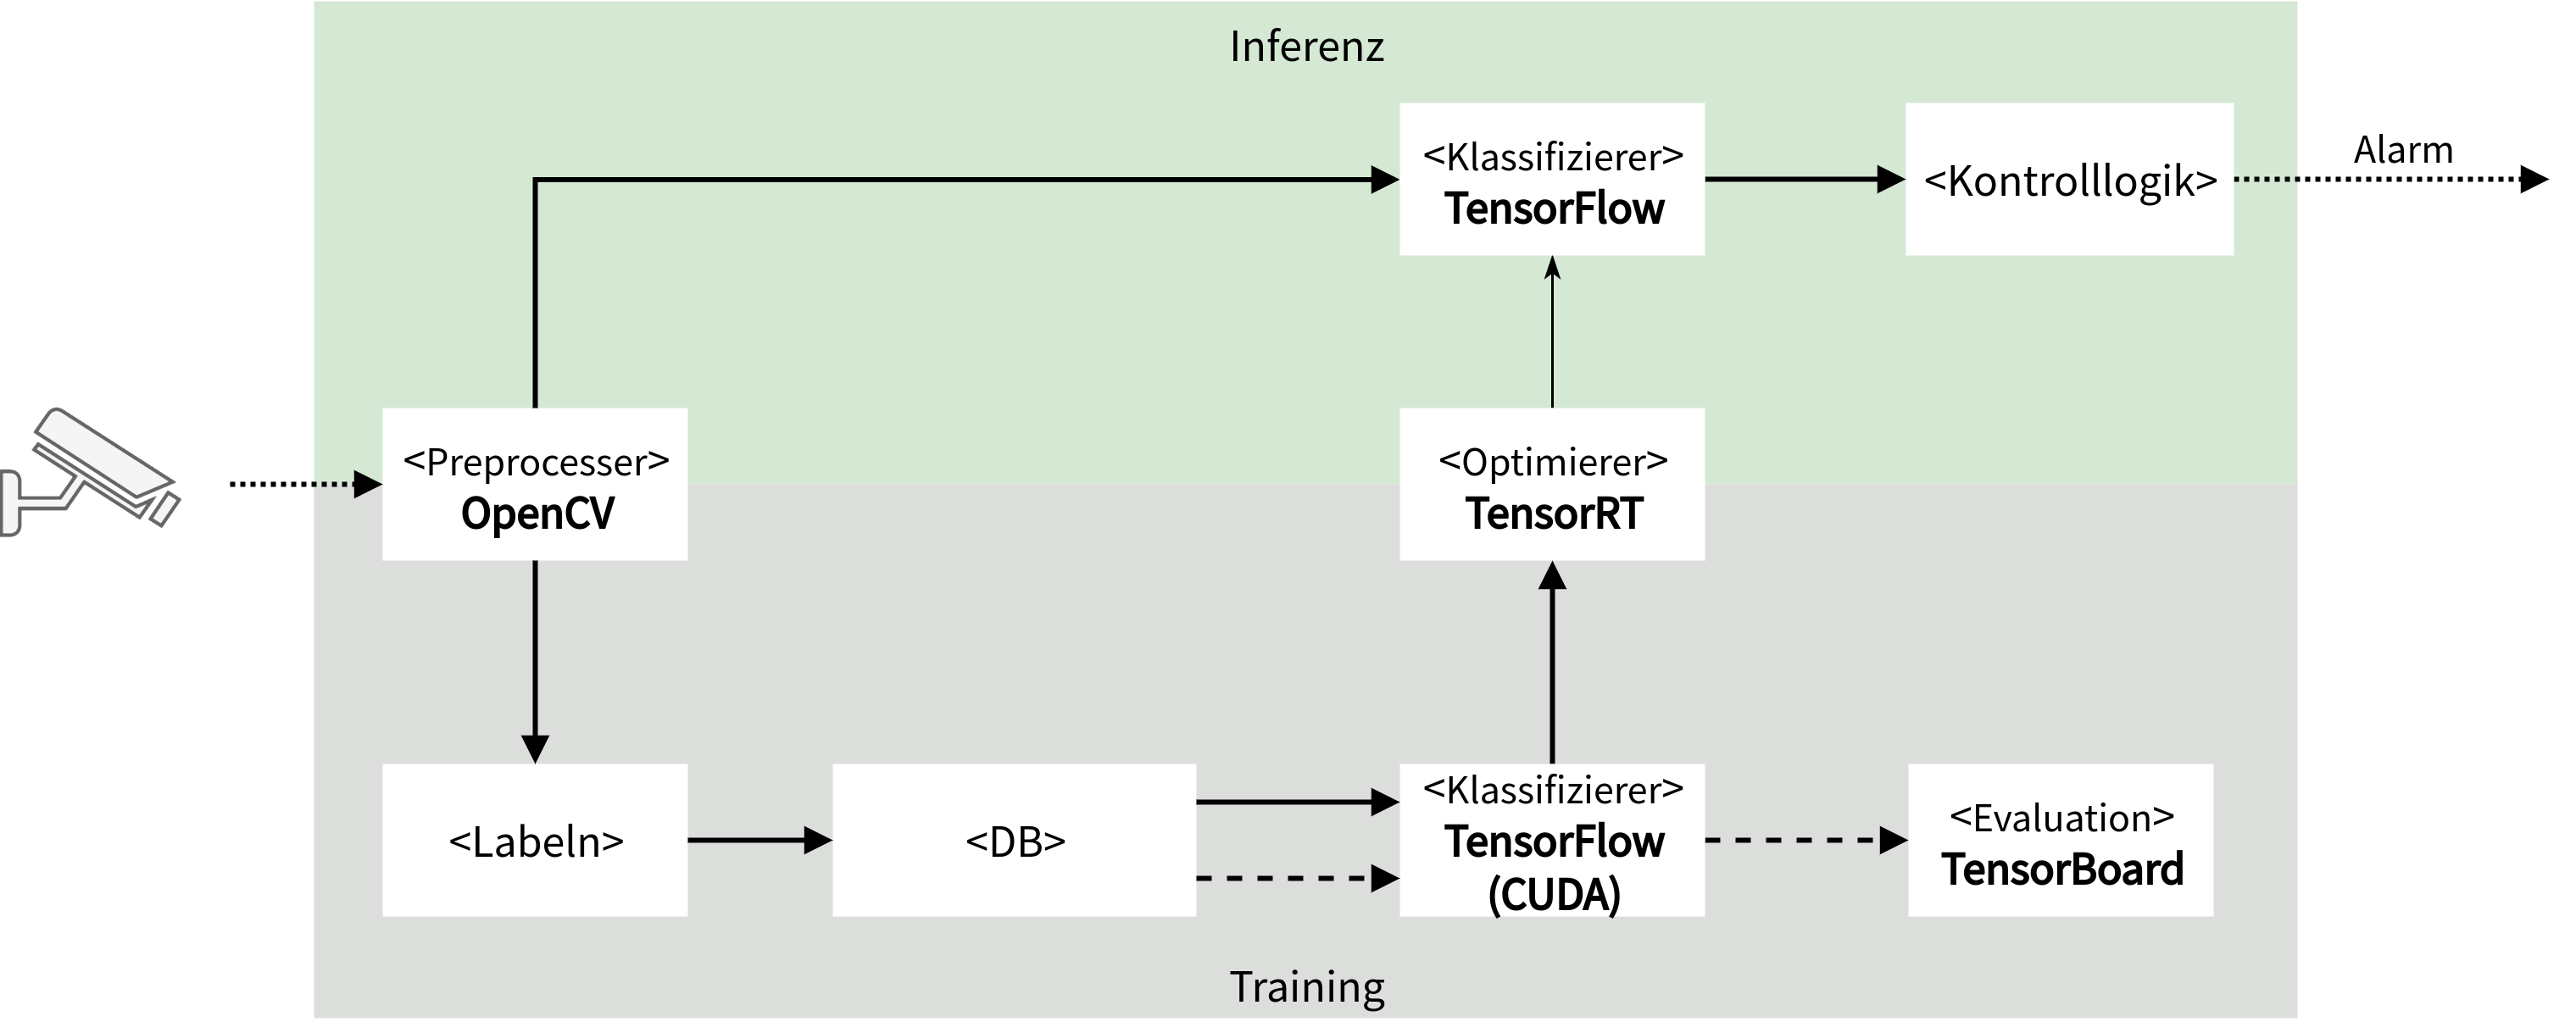
\includegraphics[width=0.95\textwidth]{figures/architecture/technologie.png}
        \end{center}
        \caption{Datenfluss \& verwendete Technologien}
        \label{ch5:fig:technologies}
    \end{small}
\end{figure}

Es wurde sich für diese Bibliotheken entschieden, da sie eine Anbindung zu \SC{Python} bieten und zu den etabliertesten zählen.
% - TensorRT (Inference)}

% ****************************************************************************************************
\section{Identifizieren von ROIs mittels Background Subtraction} \label{ch5:rois}
Für die Background Subtraction wird BMOG verwendet\footnote{Alternativ können in \SC{bgslibrary} eine Vielzahl an Algorithmen zur Background Subtraction gefunden werden \cite{sobral_bgslibrary:_2013}.}.
Die Implementierung der Autoren von BMOG ist eine Anpassung der MOG2 Variante aus \SC{OpenCV} 3 und ist zum jetzigen Zeitpunkt noch nicht öffentlich zugänglich, jedoch auf Anfrage erhältlich.
Der Code von BMOG kann über das Modul \SC{ctypes} in \SC{Python} eingebunden werden.

Für die Parameter wurden die gleichen Werte verwendet, die auch für den \SC{ChangeDetection 2014} Datensatz eingesetzt wurden.

Zur Initialisierung der Gausschen Verteilungen werden jeweils die ersten fünf Bilder einer Sequenz verwendet.

Ist das Backgroundmodell initialisiert, wird für ein neues Bild eine Vordergrundmaske erstellt.
In der Vordergrundmaske sind alle Bewegungen weiß, starre Bereiche schwarz.
Aus der binären Maske werden dann die relevanten \acp{ROI} extrahiert.
Typischerweise werden dazu zuvor die morphologischen Operatoren \IT{Open} und \IT{Close} angewandt, um einzelne Pixel zu entfernen und kleine Löcher innerhalb der Regionen zu schließen.
Diese Schritte geschehen bereits im internem BMOG Ablauf.
Die Konturen der Objekte werden mit der \SC{OpenCV} Funktion \TT{findContours} gefunden.
% Diese basiert auf dem Algorithmus von \citeauthor{suzuki_topological_1985} \cite{suzuki_topological_1985}.

Für alle gefundenen Konturen wird daraufhin eine Blobanalyse ausgeführt, in der geprüft wird, ob sie eine gewisse Größe aufweisen.
So können bereits kleinere Störungen herausgefiltert werden, da diese die Mindesthöhe und \mbox{-breite} nicht erreichen.
Ebenso wird geprüft, ob die Kontur ein passendes Seitenverhältnis aufweist.

\bigskip
\autoref{ch5:fig:bgs_blob} zeigt das Ergebnis einer Blobanalyse.
Alle roten Rechtecke sind die \acp{ROI} für die weitere Verarbeitung.

\begin{figure}[ht]
    \begin{small}
        \begin{center}
            \includegraphics[width=0.95\textwidth]{figures/ch4_bgs/combo}
        \end{center}
        \caption[Beispielhafte Blobanalyse]{Beispielhafte Blobanalyse - links: vernebelte Eingangsbilder; rechts: markierte Vordergrundmaske}
        \label{ch5:fig:bgs_blob}
    \end{small}
\end{figure}


% ****************************************************************************************************
\section{Trainingsdaten für das CNN erzeugen}
\label{ch5:data}
Um das \ac{CNN} zu trainieren, müssen die \acp{ROI} ausgeschnitten und sortiert werden.

\citeauthor{hu_finding_2016} haben gezeigt, dass zusätzlicher \IT{Kontext} beim Identifizieren von kleinen Objekten hilft \cite{hu_finding_2016}.
Deshalb wird jede \ac{ROI} um \SI{10}\% gepadded.

Anschließend müssen die extrahierten Vordergrundobjekte zwischen~
\begin{enumerate*}[(\arabic*)]
    \item \SC{landwirtschaftlichen Maschinen} und
    \item \SC{anderem}
\end{enumerate*}
unterschieden und dementsprechend sortiert werden.
Handelt es sich um sehr große Datenmengen, kann bereits auf einer Teilmenge der sortieren Bilder ein \ac{CNN} trainiert werden, welches die restlichen Bilder vorsortiert.

\bigskip
Zuletzt werden die Daten noch in drei einzelne Datensätze aufgeteilt \IT{(Holdout Methode)}:
\begin{itemize}
    \item{Der Trainingsdatensatz
        wird für das Trainieren des \ac{CNN}s verwendet.
        Die gleichen Trainingsdaten können dabei für unterschiedliche Modelle verwendet werden.}
    \item{Der Validationsdatensatz
        wird für die Optimierung des \ac{CNN}s verwendet, also für die Wahl des Modells und seiner Parameter.
        Das hat jedoch den Nachteil, dass das Modell auf diesen Datensatz angepasst wird und daher ein weiterer Datensatz für die Evaluation notwendig ist.}
    \item{Der Testingdatensatz
        wird genutzt, um das Modell auf ungesehenen Daten zu evaluieren.
        Dieser Datensatz wird nur einmalig für das finale Modell genutzt. } 
\end{itemize}

\begin{figure}[ht]
    \begin{small}
        \begin{center}
            \tikzset{
    train/.style={
        text=black,
        draw,
        minimum height=1cm,
        minimum width=6cm,
        fill=RoyalBlue!30!white},
        % left color=royalblue!30!white, right color=orange!30!white,shading angle=90},
    val/.style={
        draw,
        text=black,
        minimum height=1cm,
        minimum width=2cm,
        fill=RoyalBlue!60!white},
        % left color=orange!60!white, right color=orange!60!white,shading angle=90},
    test/.style={
        draw,
        text=black,
        fill=RoyalBlue,
        minimum height=1cm,
        minimum width=2cm}}
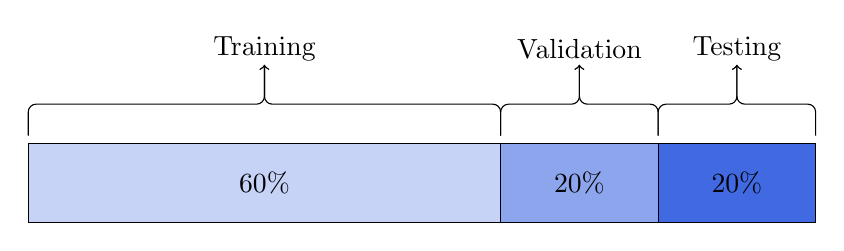
\begin{tikzpicture}[thin,black]
\path
(0,0)       node[train] (N) {60\%}
++(0:4)     node[val] (C) {20\%}
+(0:2)    node[test] (O) {20\%};
\draw[->,rounded corners=1mm] (-3.0,0.6) |- (0,1) -- ++(0,0.5);
\draw[->,rounded corners=1mm] (3.0,0.6) |- (0,1) -- ++(0,0.5);
\draw[->,rounded corners=1mm] (3.0,0.6) |- (4.0,1) -- ++(0,0.5);
\draw[->,rounded corners=1mm] (5.0,0.6) |- (4.0,1) -- ++(0,0.5);
\draw[->,rounded corners=1mm] (5,0.6) |- (6.0,1) -- ++(0,0.5);
\draw[->,rounded corners=1mm] (7,0.6) |- (6.0,1) -- ++(0,0.5);
\node at (0,1.7) {Training};
\node at (4.0,1.7) {Validation};
\node at (6.0,1.7) {Testing};
\end{tikzpicture} 
        \end{center}
        \caption{In der Praxis häufig gewählte Aufteilung der Daten}
        \label{ch5:fig:datasplit}
    \end{small}
\end{figure}

In \autoref{ch5:fig:datasplit} ist eine typische Aufteilung gezeigt \cite{suthaharan_machine_2016}.
Da für dieses Konzept jedoch nicht nur das \ac{CNN} evaluiert werden muss, sondern die Kombination mit \ac{BGS}, wird auf die Erstellung eines klassischen Testsets verzichtet.
Stattdessen werden Anfangs komplette Bildsequenzen für die Evaluation beiseite gelegt, auf denen die Kombination beider Komponenten evaluiert wird.
Es wird daher eine 75-25 Aufteilung der extrahieren \acp{ROI} verwendet.

% Ebenfalls können den Daten Bilder von z.B. \textsc{Google} oder \textsc{ImageNet}\footnote{Beispielhaft sind Traktoren, Pflanzen \& Tiere auf \textsc{ImageNet} unter den \IT{SysnetIDs} \TT{n04465501, n12513613, n00015388} zu finden} hinzugefügt werden.
% Für den Prototypen wurde sich vorerst allerdings dagegen entschieden, da hohe Differenzen in Granularität der Modelle und des Blickwinkels zu erwarten sind.


% ****************************************************************************************************
\section{Klassifikation der ROIs mittels CNNs} \label{ch5:cnn}
Zur Klassifikation der \acp{ROI} wird die Implementierung der Autoren von EfficientNet eingesetzt \cite{yakubovskiy_qubvel/efficientnet_2019}.

Anstatt, wie die Autoren, das Basismodell \TT{B0} hoch zu skalieren, wird es herunter skaliert, um noch kleinere Modelle zu erhalten.
Dies ist beispielhaft bis zu einem negativen Koeffizienten von $\phi=-6$ in \autoref{ch5:tab:efn_coeff} gezeigt.
Für die \IT{kleinen} Modelle gibt es keine Pre-Trained Gewichte, sodass sie von vorne trainiert werden müssen.

Als größtes Modell wird jenes gewählt, bei dem die Eingangsgröße des Modells der durchschnittlichen Größe der extrahierten \acp{ROI} entspricht.
Ausgehend davon werden weitere kleinere EfficientNets erstellt, um ein möglichst leichtgewichtiges Modell zu erhalten.

\begin{table}[ht]
    \tcsethrule {}{\hline \hline}{\hline}
    \tcsetcoltype[||]{c||cc|cc}{c}
    \vtablecalc[4]{$\phi$}{p=-1,-2,-3,-4,-5,-6}
                {$r=1.1.5^\phi$}{round (1.15 ^ p, 2)}
                {\BF{Auflösung:} $224*r$}{round(224 * round(1.15 ^ p, 2),0)}
                {\BF{Breite:} $w=1.1^\phi$}{round (1.1^p,2)}
                {\BF{Tiefe:} $d=1.2^\phi$}{round (1.2^p,2)}
    \caption{EfficientNet Skalierung bei negativen Koeffizienten $\phi$}
    \label{ch5:tab:efn_coeff}
\end{table}

\bigskip
Da für den Anwendungsfall vorerst nur wichtig ist, ob es sich um eine landwirtschaftliche Maschine handelt oder nicht, besteht der letzte \ac{FC} Layer nur aus einem Neuron mit der Sigmoid Aktivierungsfunktion.
Handelt es sich also beim Eingangsbild um einen Traktor, wird sich die Ausgabe idealerweise dem Wert $1$ annähern, umgekehrt dem Wert $0$.


\subsection*{Laden und Vorverarbeiten der Daten}
Bevor das \ac{CNN} trainiert werden kann, müssen die Daten geladen werden.
Der \TT{ImageGenerator} von \SC{TensorFlow} bietet neben Laden und Anpassen der Größe weitere Funktionen an.
So werden die Eingangsbilder für eine größere Vielfalt bis zu \SI{20}{\degree} rotiert und zufällig vertikal \& horizontal gespiegelt.

Zusätzlich werden, wie für die \IT{großen} EfficientNets, die Eingangsbilder normalisiert, sodass die Pixelwerte gleichmäßig verteilt sind.
Dadurch soll das \ac{CNN} schneller konvergieren.
Die \IT{Torch-Normalisierung} besteht aus drei Schritten:
\begin{enumerate}
    \item Der initiale Wertebereich $[0,255]$ wird auf $[0,1]$ verkleinert, indem alle RGB-Pixel durch $255$ geteilt werden.
    \item Den skalierten Pixeln wird der Mittelwert aller Bilder der \SC{ImageNet} Sammlung abgezogen, diese sind $0.485, 0.456, 0.406$ für die jeweiligen RGB-Channel.
    \item Zuletzt wird das Ergebnis von Schritt 2 durch die Standardabweichung der Sammlung geteilt, welche $0.229, 0.224, 0.225$ (RGB) sind.
\end{enumerate}

\subsection*{Training} \label{ch5:cnn:train}
Die Lernrate ist eine der wichtigsten Parameter beim Training eines \ac{ANN}s.
Ist die Lernrate zu klein, trainiert das \ac{ANN} nur sehr langsam.
Ist die Lernrate zu groß, kann es passieren, dass zu drastische Anpassungen ausgeführt  werden und das \ac{ANN} sogar schlechter wird.
Dieses Verhalten ist in \autoref{ch5:fig:lr_expl} zu sehen.

\begin{figure}[ht]
    \begin{small}
        \begin{center}
            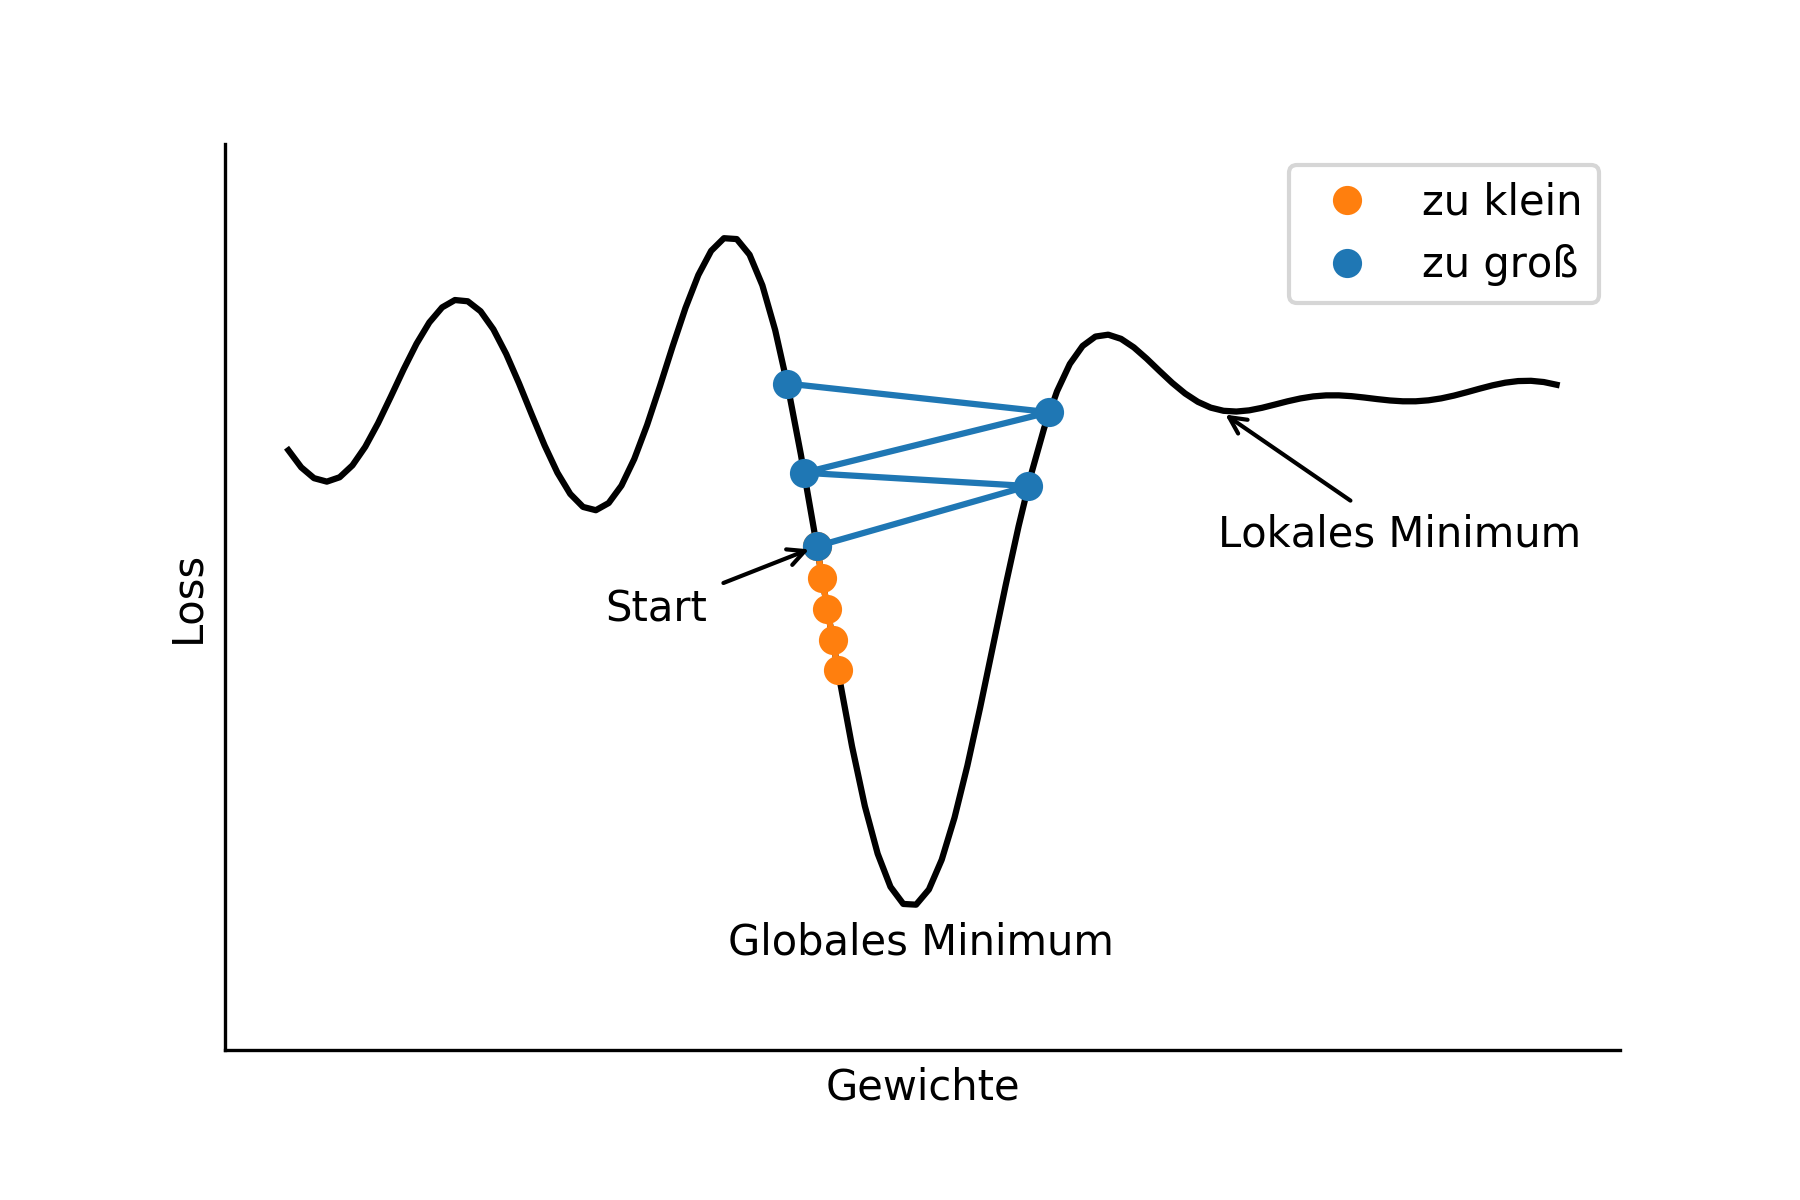
\includegraphics[width=0.95\textwidth]{figures/ch5/lr_big_small}
        \end{center}
        \caption{Lernrate Exploration}
        \label{ch5:fig:lr_expl}
    \end{small}
\end{figure}

Die optimale Lernrate liegt also in der Mitte.
Jedoch kann es dann leicht passieren, dass das \ac{ANN} in einem Lokalem Minimum stecken bleibt.

An dieser Stelle setzt die zyklische Lernrate an \cite{smith_cyclical_2017}.
Dabei pendelt die Lernrate zwischen einem minimalem und maximalem Wert hin und her.
Beim Erhöhen der Lernrate kann es so zu kurzzeitigen Verschlechterungen kommen, allerdings kann dabei aus kleinen Lokalen Minima \IT{rausgeklettert} werden, sodass sich Langzeit eine positive Entwicklung ergibt.

Zum Bestimmen der minimalen und maximalen Lernrate wird ein Range Test durchgeführt, bei dem das Modell für mehrere Epochen mit linear wachsenden Lernraten trainiert wird.
Das Minimum entspricht dem Wert, bei dem das Modell anfängt zu lernen, also die Genauigkeit steigt und der Loss sinkt.
Das Maximum ist erreicht, sobald die Genauigkeit abflacht, sich verschlechtert oder anfängt zu fluk­tu­ie­ren. 

Sind die zwei Parameter bestimmt, werden die \acp{CNN} für $100$ Epochen trainiert.
Empfohlen wird, dass die Lernrate alle $4$ bis $20$ Epochen einen Zyklus vollendet, deshalb wird für dieses Konzept die Mitte von $10$ gewählt.

Das Training wird früher beendet, wenn sich der Loss vom Validationsdatensatz über $25$ Epochen nicht verbessert \IT{(Early Stopping)}. 
So soll das Modell regularisiert werden, da wenn sich der Trainings Loss zwar stets verbessert, der Validations Loss jedoch nicht, davon auszugehen ist, dass das Modell nicht mehr generalisiert bzw. overfittet.

Da es sich um ein binäres Klassifikationsproblem handelt, wird der \IT{Binary Crossentropy} Loss verwendet.

% - !kein! K-Fold, da groesser Datensatz und \"missing something important\" unwahrscheinlich und computing overhead sehr gross \\
% wenn doch: \\
% \begin{minted}[linenos,frame=lines,framesep=2mm,breaklines,tabsize=4]{python}
% # dir in k-folds aufteilen
% for i in range(k_folds):
%     train.flow_from_directory(data_path=dir-fold-{i}, subset='training')
%     val.flow_from_directory(data_path=dir-fold-{i}, subset'validation')

%     model = build_model_x()
%     history = model.fit_generator(generator=train, validation_data=val)

%     train_acc.append(history['acc'])
%     val_acc.append(history['val_acc'])
% \end{minted}


% No, and it’s not something you’re likely to do with a deep learning model.

% Cross validation is most useful when the dataset is relatively small (hundreds, maybe thousands of training examples). When the dataset is large, training can already take hours. Using cross validation will result in multiplying the training time by the number of folds, but won’t give you much benefit.

% The reason cross validation is useful is because when you have a small number of examples to work with, you run the risk of “missing something important” when you’re unable to train on 20% of your data because you’re using it for testing. But as the dataset size increases, you are statistically less likely to encounter this problem.

% Deep learning models only really make sense when you have a lot of training data to work with. So if your dataset is small enough that you can afford to use cross validation, you’re probably overfitting and should use a less complex model than what TensorFlow will give you.

% \section{Optimieren des CNNs und Inferenz}
% - TensorRT: pruning, gpu operator, fp
% - Inferenz: BGR/RGB, Preprocessing

% ****************************************************************************************************
\section{Kontrolllogik für Alarm}
\label{ch5:alarm}
Für die Alarmgabe muss eine Kontrolllogik erstellt werden, welche auf die Vorhersagen des \ac{CNN}s reagiert.
Schlägt der Alarm aus, soll an den Windparkbetreiber eine Email gesendet werden, woraufhin dieser das Windrad stoppt.

Intuitiv gilt, dass wenn ein Traktor in mehreren Bildern erkannt wird, seine tatsächliche Anwesenheit wahrscheinlicher ist.
Wird hingegen ein Traktor nur in einem von vielen Bildern erkannt, ist es wahrscheinlich eine Fehlprognose.
Deshalb werden in beiden folgenden Ansätzen die Vorhersagen über mehrere Bilder aggregiert betrachtet.

\bigskip
Für beide Ansätze gelten folgende Definitionen:
\begin{description}
    \item[Schwellwert $\tau_1$] 
        setzt die Grenze, ab welcher Alarm gegeben wird.
    \item[Anzahl der Bilder $F_N$] 
        gibt die Anzahl der zu betrachtenden Bilder an.
    \item[Vorhersagen $P$ \& $p$]
        geben die Wahrscheinlichkeiten der Klassifikation für eine bestimmte \ac{ROI} an.
        Diese liegen zwischen $[0,1]$. Je größer $p$, desto wahrscheinlicher handelt es sich um eine landwirtschaftliche Maschine.
        $P$ sind alle Wahrscheinlichkeiten eines Bildes.
\end{description}

Dabei ist $F_N$ abhängig von~
\begin{enumerate*}[(\arabic*)]
    \item der Mahdgeschwindigkeit, welche durch Mähwerk und Bodenbeschaffenheit bestimmt wird, und
    \item der Bildwiederholungsrate der Kamera.
\end{enumerate*}

Fährt ein Traktor beispielhaft mit $30$ km/h über das $300$ Meter lange Feld, durchquert er es bereits in $36$ Sekunden.
Wenn er zusätzlich $10$ Sekunden zum Wenden braucht und in Sekunde $46$ erneut beschleunigt, wird er innerhalb einer Minute in vielen unterschiedlichen Winkeln aufgezeichnet.
So sollte eine zuverlässige Vorhersage nach einer Minute getroffen werden können.

Wenn die Kamera alle $3$ Sekunden ein Bild macht, ergibt sich eine Bildanzahl von $F_N=20$.

\subsection{Ansatz 1}
Im erstem Ansatz werden die maximalen Vorhersagen der einzelnen Frames aufsummiert und durch die Anzahl der Frames geteilt.

\begin{flalign}
    T &= \frac{1}{F_N} \cdot {\sum_{n=1}^{F_N}{max(P_n)}}
\end{flalign}

Anschließend wird Alarm bei $T \geq \tau_1$ gegeben.


\subsection{Ansatz 2}
Es gelten zusätzlich folgende Definitionen für Ansatz 2:
\begin{description}
    \item[Schwellwert $\tau_2$]
        wird genutzt, um einzelne Vorhersagen einzuordnen.
        Ist die Vorhersage niedriger als der Schwellwert, gilt diese Vorhersage nicht als landwirtschaftliche Maschine.
    \item [Anzahl $N$]
        entspricht der Anzahl aller Vorhersagen der letzten $F_N$ Frames, deren Wahrscheinlichkeiten größer $\tau_2$ sind.
\end{description}

Für den zweiten Ansatz werden die einzelnen Vorhersagen über ihre räumlichen Koordinaten gruppiert.
So können die Pfade der Objekte nachvollzogen werden.
Die maximale Euklidische Distanz\footnote{Die Euklidische Distanz wird mittels Pythagoras bestimmt: $\sqrt{(x_1-x_2)^2 + (y_1-y_2)^2}$}, um zwei Punkte zu gruppieren, ist dabei von der Bildwiederholungsrate und der Geschwindigkeit der Objekte abhängig.

Eine Vorhersage wird einem Pfad hinzugefügt, falls diese die maximale Distanz zum neustem Punkt des Pfades unterschreitet.
Dabei werden nur Vorhersagen betrachtet, deren Wahrscheinlichkeiten größer $\tau_2$ sind.

\begin{figure}[ht]
    \begin{small}
        \begin{center}
            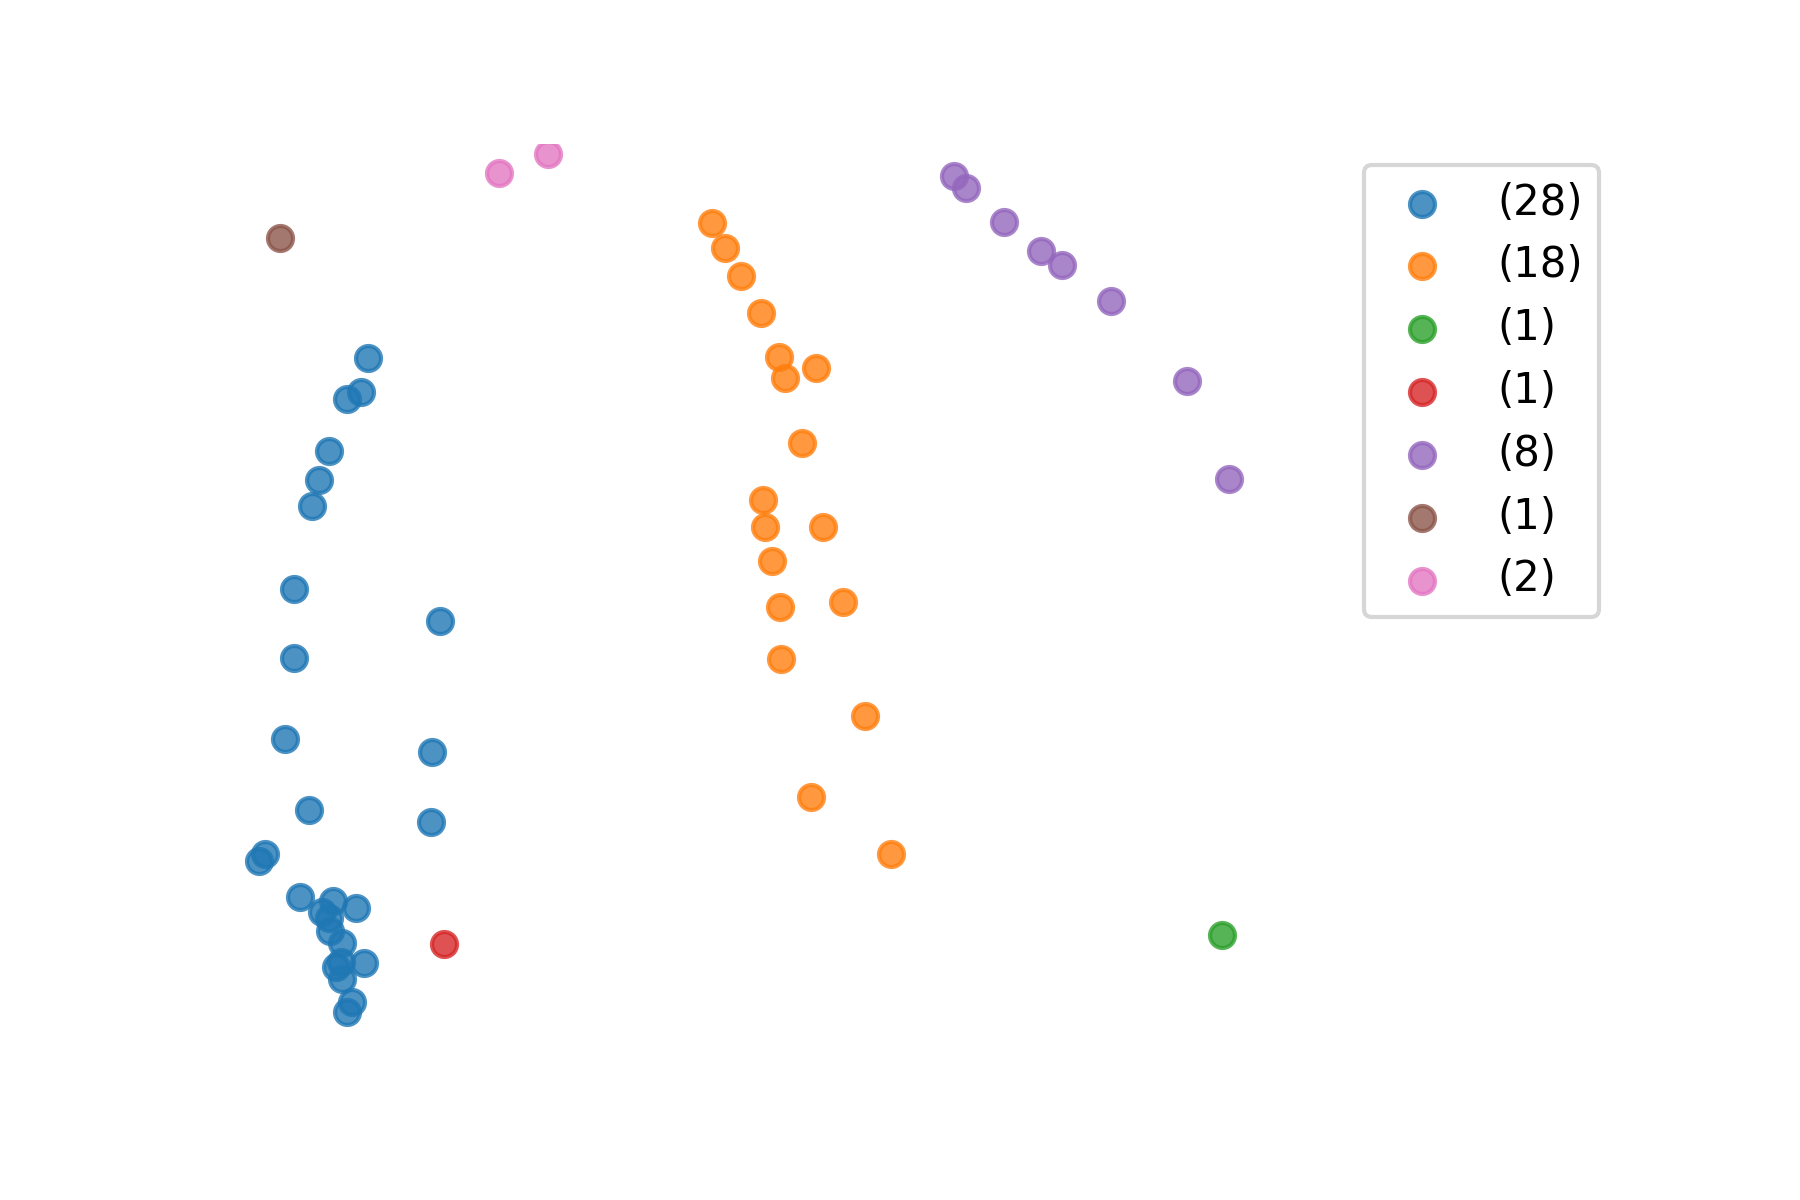
\includegraphics[width=0.95\textwidth]{figures/ch5/predicted_path}
        \end{center}
        \caption{Pfade über Euklidische Distanz gruppiert}
        \label{ch5:fig:pred_path}
    \end{small}
\end{figure}

\bigskip
In \autoref{ch5:fig:pred_path} ist eine beispielhafte Gruppierung zu sehen.
Jeder Punkt stellt dabei eine Vorhersage da, für die $p > \tau_2$ gilt.
Die Farben markieren die Gruppenzugehörigkeiten.

Sind die Vorhersagen einem Pfad zugeordnet, kann eine \gls{hysterese} Funktion eingeführt werden, die lange Pfade (z.B. Blau) stärker gewichtet und einzelne Punkte (z.B. Grün) schwächer.
So können die Wahrscheinlichkeiten zum Beispiel mit der Länge ihres zugehörigen Pfades multipliziert werden:

\begin{flalign}
    T &= \frac{1}{N} \cdot \sum_{i=1}^{N}{p_i \cdot ||pfad(p_i)||}
\end{flalign}

Auch hier wird bei $T \geq \tau_1$ Alarm gegeben.